\chapter{How I Turned \$1{,}000 Into \$1 Billion}

These notes follow a School of Hard Knocks interview with Glen Boyd, curated for this volume by LazyingArt LLC. The source is an interview, not a blackboard lecture, so the mathematics here is a disciplined reconstruction of the commercial mechanism the speaker is describing: a technical engine, a market shift, a proof-of-use test, and then a second round of scaling problems in capital, management, and life. The interview itself opens with the result before the explanation, and the chapter should preserve that rhythm.

\section{Outcome First, Then Origin}

The lecture begins by handing us the answer before the argument. That is the first important structural fact. We are told what happened before we are told why it happened:
\begin{align}
R_{1\,\mathrm{mo}} &= \$50{,}000,\\
R_{11\,\mathrm{mo}} &\approx R_{\mathrm{security}},\\
S_{4\,\mathrm{yr}} &= \$120\,\mathrm{M}.
\end{align}

The first line says the pivoted company did real business immediately, and did it without advertising. The second says that within eleven months the new business was already approaching the scale of the legacy security company. The third gives the long payoff: four years later the business was doing \$120 million in sales. The rest of the lecture is a reconstruction of how those three lines could become true.

Only after this numerical hook do we rewind. Boyd describes teaching himself to program, starting a technology company in his early twenties, taking it public in 1999, and later selling it in a merger. The biographical point is not merely that he was early. It is that he was early inside a network transition and had already learned how to build real software for serious customers.

That matters because the first company was not a toy. Before the pivot, the business already had the Federal Reserve, almost every major bank in the United States, and a very small team operating out of a little office while producing roughly a million dollars a year. So when the lecture turns to the pivot, it is not the story of a failed founder searching for his first break. It is the story of a working business deciding that the ground beneath it is changing.

\section{From Security Product to Internet Pivot}

The original product was a security product for internal networks. Banks and financial institutions were being pushed toward audit controls as more of their work became computerized, and Boyd's product logged and analyzed traffic on local area networks. The lecture is careful here: the first business already solved a real institutional problem.

\subsection{Question \& Answer}

\paragraph{Question.} How did he know this was the company to go all in on?

\paragraph{Answer.} He did not know the final company at the beginning. The interview answers the question by destabilizing it. What was worth trusting was not a perfectly finished idea, but a strong technical capability together with the willingness to redirect it when the market changed. The company becomes worth going all in on when the founders see that the original product is not the last product.

That market change arrives with the internet. Yahoo and Netscape are not just historical color. In the lecture they are regime-change markers. The world is no longer being organized only as internal networks inside institutions; it is becoming networked in public. Boyd's train metaphor is therefore more than rhetoric. He sees the future already moving and asks whether the company can still catch the last car.

This is why the lecture spends time on the summer of uncertainty. The founders are not polishing a pitch deck. They are trying to decide whether they are willing to leave behind a successful, concentrated business in order to participate in the larger network world that is coming into view.

\section{Same Engine, New Output}

The pivot itself is conceptually clean. The firm keeps the analytic engine it has already built, but changes both the domain of the incoming data and the kind of report it emits. Let \(A\) denote the existing traffic-analysis engine, \(T_{\mathrm{LAN}}\) internal network traffic, and \(T_{\mathrm{web}}\) anonymous inbound web traffic. Then the lecture can be written, cautiously, as
\begin{align}
A(T_{\mathrm{LAN}}) &\mapsto \mathcal{R}_{\mathrm{sec}},\\
A(T_{\mathrm{web}}) &\mapsto \mathcal{R}_{\mathrm{mkt}}.
\end{align}

Here \(\mathcal{R}_{\mathrm{sec}}\) is a security or fraud-oriented report, while \(\mathcal{R}_{\mathrm{mkt}}\) is a marketing or audience-interest report. This is the chapter's central reconstruction. The engine remains; the question changes.

\begin{figure}[h]
\centering
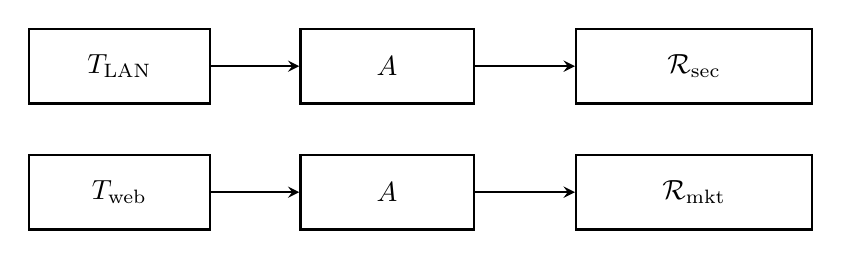
\begin{tikzpicture}[>=stealth,thick]
\node[draw,rectangle,minimum width=2.3cm,minimum height=0.95cm] (lan) at (0,1.6) {$T_{\mathrm{LAN}}$};
\node[draw,rectangle,minimum width=2.2cm,minimum height=0.95cm] (a1) at (3.4,1.6) {$A$};
\node[draw,rectangle,minimum width=3.0cm,minimum height=0.95cm] (sec) at (7.3,1.6) {$\mathcal{R}_{\mathrm{sec}}$};

\node[draw,rectangle,minimum width=2.3cm,minimum height=0.95cm] (web) at (0,0) {$T_{\mathrm{web}}$};
\node[draw,rectangle,minimum width=2.2cm,minimum height=0.95cm] (a2) at (3.4,0) {$A$};
\node[draw,rectangle,minimum width=3.0cm,minimum height=0.95cm] (mkt) at (7.3,0) {$\mathcal{R}_{\mathrm{mkt}}$};

\draw[->] (lan) -- (a1);
\draw[->] (a1) -- (sec);
\draw[->] (web) -- (a2);
\draw[->] (a2) -- (mkt);
\end{tikzpicture}
\caption{A cautious reconstruction of the pivot described in the lecture: the analytic core is held fixed while the traffic source and report type change.}
\end{figure}

The Sports Illustrated example makes this operational. The early web customer does not merely want a count of total hits. He wants to know what kind of audience is present. Let \(U\) denote the number of unique visitors, \(f\) the repeat-visit frequency, and \(V\) the total visit count. Then the relevant arithmetic is
\begin{equation}
V = U\cdot f.
\end{equation}

The point is not that this formula is profound. The point is that equal traffic totals can hide radically different audience structures. Boyd's example can be written as
\begin{align}
100{,}000\times 1 &= 100{,}000,\\
10{,}000\times 10 &= 100{,}000.
\end{align}

The same total visits may mean many distinct people arriving once, or a much smaller population returning repeatedly. For a marketer, those are different worlds.

\paragraph{Worked example.} If we compare
\[
(U,f)=(100{,}000,1)
\qquad\text{and}\qquad
(U,f)=(10{,}000,10),
\]
then the raw total \(V\) is unchanged while the inferred market reality is not. The first case suggests breadth; the second suggests intensity. This is exactly why the output of the system changes from a fraud report to a marketing report. The engine had already learned to detect structure in large traffic streams. The pivot taught it to answer a new commercial question.

\begin{figure}[h]
\centering
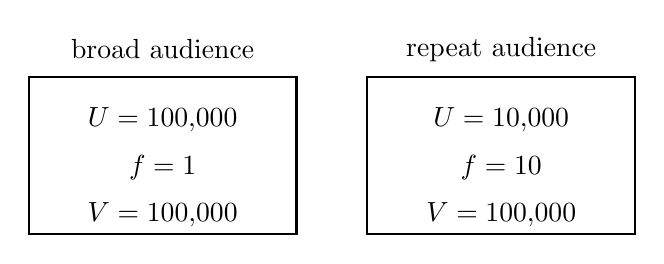
\begin{tikzpicture}[thick]
\draw (0,0) rectangle (3.4,2.0);
\draw (4.3,0) rectangle (7.7,2.0);
\node at (1.7,1.45) {$U=100{,}000$};
\node at (1.7,0.85) {$f=1$};
\node at (1.7,0.25) {$V=100{,}000$};

\node at (6.0,1.45) {$U=10{,}000$};
\node at (6.0,0.85) {$f=10$};
\node at (6.0,0.25) {$V=100{,}000$};

\node at (1.7,2.35) {broad audience};
\node at (6.0,2.35) {repeat audience};
\end{tikzpicture}
\caption{Equal traffic totals can hide different audience structures. The lecture's Sports Illustrated example is a counting problem before it is a marketing problem.}
\end{figure}

Now the opening numbers reappear with force. The lecture has just told us that the founders did not know in advance whether the dogs would eat the dog food. The answer came quickly: \$50,000 in the first month, without advertising; near-parity with the old company within eleven months; \$120 million in sales within four years. Those numbers are not decorative. They are the proof that the remapping worked.

\section{Proof Before Funding}

Only after the pivot has been validated does the host turn to funding. This order matters. The lecture does not begin with capital. It begins with evidence.

\subsection{Question \& Answer}

\paragraph{Question.} How do we get funding when all we have is an idea?

\paragraph{Answer.} We do not stay at the level of the idea any longer than necessary. In the lecture the path to capital is monotone: move from concept to something demonstrable, then from demonstrable product to actual use. What investors are being asked to fund is not merely imagination, but an observed reaction from the market.

A compact reconstruction is
\begin{equation}
\text{idea}\to \text{demo}\to \text{early adoption}\to \text{investable company}.
\end{equation}

This is not a law of nature, but it is the logic of the interview. The weaker the evidence, the more one is asking for belief. The stronger the evidence, the more the market has already begun to speak for itself.

\begin{figure}[h]
\centering
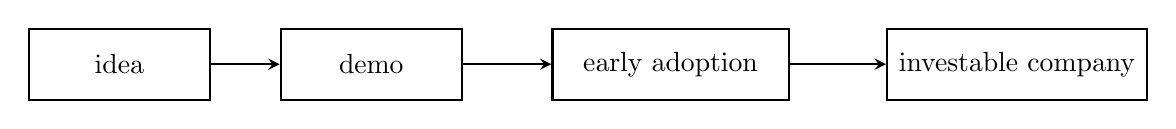
\begin{tikzpicture}[>=stealth,thick]
\node[draw,rectangle,minimum width=2.3cm,minimum height=0.9cm] (i) at (0,0) {idea};
\node[draw,rectangle,minimum width=2.3cm,minimum height=0.9cm] (d) at (3.2,0) {demo};
\node[draw,rectangle,minimum width=3.0cm,minimum height=0.9cm] (e) at (7.0,0) {early adoption};
\node[draw,rectangle,minimum width=3.3cm,minimum height=0.9cm] (c) at (11.4,0) {investable company};
\draw[->] (i) -- (d);
\draw[->] (d) -- (e);
\draw[->] (e) -- (c);
\end{tikzpicture}
\caption{The lecture's funding logic: capital follows proof more readily than it follows aspiration.}
\end{figure}

This is where the old dog-food expression enters. It is not just a slogan. It is the interview's criterion for market truth. However elegant the advertising, if the dogs do not eat the dog food, the product has not crossed the first threshold.

The lecture then gives examples that are intentionally small at the beginning. YouTube begins with cat videos. Instagram begins with people sharing personal photos. The point is not that the starting use-case is lofty. The point is that it is usable, and therefore capable of generating real pull.

\begin{figure}[h]
\centering

\includegraphics[width=0.62\textwidth]{lecture_132_figure_03.png}
\caption{Instagram shown as an early example of a simple use-case, personal photo sharing, that became important because users actually wanted it.}
\end{figure}

The retained frame is useful precisely because it is ordinary. We do not need to extract tiny interface text from it. Its evidentiary value lies in the visible narrowness of the initial use-case. A small use-case that people genuinely adopt is better evidence than a grand abstraction that nobody touches. This is what the lecture means when it says the dogs love the dog food.

\section{Balance, Partnership, and Risk on the Line}

Once the product has become real, the lecture widens. It moves from business proof to founder capacity. This is not a digression. It is the next scaling problem.

Boyd speaks about life-work balance, then about life-health-work balance. He describes divorce early in life, later serious health consequences, and the basic entrepreneurial tendency to continue working because one loves the work even when the people around one cannot fully share that absorption. The business is growing, but so is the pressure on the human being carrying it.

The lecture's first operational remedy is partnership. A good partner is not merely emotional support. A partner is a second load-bearing element in the system. Tasks can be divided; emergencies can be covered; arguments can be used to test decisions rather than avoided out of politeness; distinct skill sets can be combined into a wider competence than either founder has alone.

That line of thought prepares the risk story. Boyd describes quitting his job, getting down to roughly the last \(\$1{,}000\) in his bank account, selling his motorcycle to extend the runway, and then being carried a little farther by his partner's personal money. The transcript becomes garbled immediately after the phrase ``not an understatement,'' so the chapter should not force detail there. But the stable logic is clear enough.

His risk heuristic is simple and severe: the worst likely outcome is that he has to go get a job. The more painful outcome is not failure but permanent wondering. The lecture therefore treats entrepreneurial risk not as theatrical heroism, but as a comparison between bounded downside and the irreversible cost of never having tried.

\section{Judgment Under Scale}

From this point on, the lecture becomes a sequence of operating judgments. It is useful to keep them in the order given, because the speaker is moving from hiring, to financial error, to venture capital, to scale, and only then to the abstract models that clarified the whole thing for him.

First come the traits he looks for in leadership: honesty, intelligence, and the ability to take constructive feedback. The feedback criterion is especially revealing because it includes himself. The lecture's picture of early partnership is not harmonious agreement but serious argument in search of the best path.

The worst financial decision is equally revealing. It is not described as a spreadsheet mistake. It is getting involved in a business he did not actually want to be in, against his own gut, and then having to spend years trying to salvage it before losing close to \(\$3\,\mathrm{M}\). The lesson is less ``do not lose money'' than ``do not volunteer your life into an enterprise you do not believe in.''

The best financial decision sounds, at first, like something else entirely. The company is profitable and growing. The founders seek venture capital to accelerate expansion. They spend substantial time in what he calls a kind of courtship. Then the investors pass. In the moment that is a rejection; in the lecture's later accounting, it becomes a hidden advantage.

\begin{figure}[h]
\centering

\includegraphics[width=0.78\textwidth]{lecture_132_figure_05.png}
\caption{Startup pitch-board imagery accompanying the discussion of venture-capital courtship. The frame is contextual evidence for the fundraising atmosphere, not a literal historical board from Boyd's company.}
\end{figure}

The screenshot is useful here not because it contains readable equations, but because it anchors the setting the lecture is describing: presentation, courtship, persuasion, and traction theater. The tiny charts on the board are unreadable and should remain unread, but the visual logic of the moment is secure.

The lecture's commercial conclusion can be compressed as
\begin{align}
\frac{dE}{ds} &> 0,\\
O_{\mathrm{founders,IPO}} &\approx 95\%.
\end{align}

The first line is schematic, not quoted. It encodes the lecture's warning that expenses scale along with the company, so one bad disturbance at larger scale can do more damage than one bad disturbance at smaller scale. The second line is a hard outcome from the interview: when the company went public, the two founders still owned about \(95\%\) of it. The venture-capital pass forced frugality and therefore preserved ownership.

\begin{figure}[h]
\centering
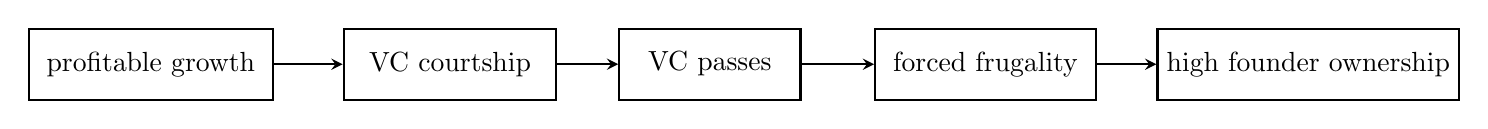
\begin{tikzpicture}[>=stealth,thick]
\node[draw,rectangle,minimum width=3.1cm,minimum height=0.9cm] (p) at (0,0) {profitable growth};
\node[draw,rectangle,minimum width=2.7cm,minimum height=0.9cm] (v) at (3.8,0) {VC courtship};
\node[draw,rectangle,minimum width=2.3cm,minimum height=0.9cm] (x) at (7.1,0) {VC passes};
\node[draw,rectangle,minimum width=2.8cm,minimum height=0.9cm] (f) at (10.6,0) {forced frugality};
\node[draw,rectangle,minimum width=3.3cm,minimum height=0.9cm] (o) at (14.7,0) {high founder ownership};
\draw[->] (p) -- (v);
\draw[->] (v) -- (x);
\draw[->] (x) -- (f);
\draw[->] (f) -- (o);
\end{tikzpicture}
\caption{The lecture's venture-capital sequence: a failed financing attempt becomes a source of discipline and preserved ownership.}
\end{figure}

\subsection{Question \& Answer}

\paragraph{Question.} Why do strong employees begin to fail when the company grows?

\paragraph{Answer.} Because the company is changing altitude while we are still judging the person as if the job were the same job. A manager who was excellent at one scale may be over threshold at the next.

Here the interview becomes explicitly model-driven. Boyd says that reading \emph{Into Thin Air} made the problem legible to him. In the mountain analogy, everyone has an altitude beyond which oxygen becomes insufficient; simple tasks become difficult, then dangerous. The company analogue is that a person hired to manage a modest load may, six or twelve months later, be trying to manage a radically larger one.

A compact reconstruction is
\begin{equation}
n>n^{*} \Rightarrow \text{manager overload and failure},
\end{equation}
where \(n\) is managerial load and \(n^{*}\) is the capacity threshold for the current person.

\begin{figure}[h]
\centering
\begin{tikzpicture}[x=1cm,y=1cm,>=stealth,thick]
\draw[->] (0,0) -- (6.6,0) node[right] {$n$};
\draw[->] (0,0) -- (0,3.7) node[above] {performance};
\draw (0.35,0.55) .. controls (1.45,1.95) and (2.4,2.75) .. (3.15,3.0);
\draw (3.15,3.0) .. controls (4.05,2.95) and (4.95,1.95) .. (6.0,0.55);
\draw[dashed] (3.65,0) -- (3.65,3.15);
\node[below] at (3.65,0) {$n^{*}$};
\end{tikzpicture}
\caption{A schematic overload threshold. As managerial load rises past $n^{*}$, a previously strong employee may begin to fail.}
\end{figure}

The juggling analogy in the lecture makes the same point more concretely. One can juggle three balls, then four, then five. But eventually the system reaches a point where everything comes down at once. That gives the manager's responsibility a precise shape: stop handing out balls, reassign responsibilities, or hire someone who has already operated above the level the role is about to require.

The second named book, \emph{Crossing the Chasm}, gives the external-market version of the same problem. Early users are not the whole market, and success with early adopters does not automatically transfer into mainstream adoption. The lecture renders this as a break in the bell curve:
\begin{equation}
\text{early adopters}\;\big|\;\text{chasm}\;\big|\;\text{early majority}.
\end{equation}

\begin{figure}[h]
\centering
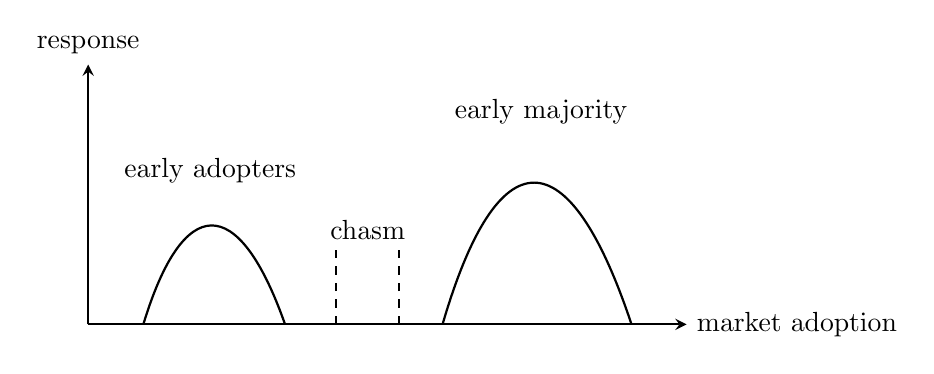
\begin{tikzpicture}[x=1cm,y=1cm,>=stealth,thick]
\draw[->] (0,0) -- (7.6,0) node[right] {market adoption};
\draw[->] (0,0) -- (0,3.3) node[above] {response};
\draw (0.7,0) .. controls (1.2,1.65) and (1.9,1.7) .. (2.5,0);
\draw (4.5,0) .. controls (5.2,2.4) and (6.1,2.4) .. (6.9,0);
\draw[dashed] (3.15,0) -- (3.15,1.0);
\draw[dashed] (3.95,0) -- (3.95,1.0);
\node at (1.55,1.95) {early adopters};
\node at (5.75,2.7) {early majority};
\node at (3.55,1.2) {chasm};
\end{tikzpicture}
\caption{A cautious sketch of the market gap invoked in the lecture's discussion of \emph{Crossing the Chasm}.}
\end{figure}

It is worth pausing on the symmetry. \emph{Into Thin Air} explains why scale breaks people inside the firm. \emph{Crossing the Chasm} explains why scale stalls in the market outside the firm. Together they give the lecture its sharpest general lesson: growth is not one problem but several, and they appear at different layers.

\section{Reflection: Happiness, Regret, and Starting Now}

Only after all of this does the lecture narrow back down to money itself. The answer to whether money buys happiness is deliberately qualified. Yes, it buys something real at the lower end: relief from poverty, basic security, the ability to educate one's children, the freedom to try things without immediate ruin. But beyond a certain point the lecture insists that marginal money stops doing the work people imagine it will do.

This closing matters because it prevents the chapter from misreading the opening figures. The \(\$120\,\mathrm{M}\) in sales and the billion-dollar exit are real facts, but they are not the lecture's final criterion of value. The interview finally turns toward how one should live with time, health, and ambition.

The younger-self advice comes as a cluster rather than a single slogan:
\begin{itemize}
\item enjoy life more and not only the work,
\item take care of health earlier,
\item avoid ambition that destroys relationships,
\item seek serious financial advice once success arrives.
\end{itemize}

Then the host adds a final prompt about people who always mean to start tomorrow. Glen's answer is the correct ending for the whole lecture. Procrastination is the enemy because time is the one nonrenewable resource. If we fail, fail fast. If we learn, learn early. Delay does not preserve optionality forever; often it only increases the distance between the present and any future success we claim to want.

\section{Summary}

The lecture unfolds in a very controlled order. First it gives us the outcome. Then it rewinds into the old business. Then it shows that the decisive act was not founding from nothing, but pivoting without discarding the analytic core. Next it argues that proof matters more than pitch, that users matter more than polish, and that a small use-case with genuine pull is the beginning of a serious company.

After that, the lecture raises the second set of problems: the founder's own life, the need for a partner, the bounded logic of risk, the pressure of expenses under scale, the preservation of ownership through frugality, the overload threshold in management, and the market threshold in adoption. By the end the story is no longer merely about having made a great deal of money. It is about recognizing how technical capability, commercial evidence, human limits, and time all interact.

So the notes should leave us with a clean sequence of mechanisms: keep the engine, change the question, let the market answer, protect the balance sheet, respect capacity thresholds, and start before delay itself becomes the hidden cost.